\newpage

\begin{figure*}
\centering
    \includegraphics[width=0.24\textwidth]{images/explicit_understanding.png}
    \includegraphics[width=0.24\textwidth]{images/explicit_meetneed.png}
    \includegraphics[width=0.24\textwidth]{images/explicit_credibility.png}
    \includegraphics[width=0.24\textwidth]{images/explicit_general.png}
    \caption{Scatter plots between 5-run mean dimension scores automatically extracted from user responses and explicit ratings given by users in the interview.\label{fig:scatter_coor}}
\end{figure*}

\begin{figure*}[t!]
    \centering
    \begin{subfigure}[]{\linewidth}
         \includegraphics[width=1\linewidth]{images/chatbot-ui.png}
    \caption{Chat with target LLMs.}
    \label{fig:target_llm_ui}
    \end{subfigure}
        \begin{subfigure}[]{\linewidth}
         \includegraphics[width=1\linewidth]{images/interviewer-ui.png}
    \caption{\method-Interviews.}
    \label{fig:clue_interviewer_ui}
    \end{subfigure}
    \caption{An example of the UIs used for the hosted LLM chat and \method-Interviewer.}\label{fig:clue_ui}
\end{figure*}



\begin{figure*}[h]
    \centering
    \small
\begin{tcolorbox}[colback=gray!1, colframe=black!50, title=Interviewer System Prompt:]

\textbf{Instructions:} You are a user experience (UX) researcher. You are going to design a UX interview and conduct the interview with a user. The product for the UX interview is a ChatBot. The user in this interview has just had a conversation with the ChatBot prior to this interview. The goal of the interview is to understand the user’s experience using the ChatBot, if the ChatBot successfully met their needs or solved their problems, and gather feedback on how to improve the ChatBot. Your interview flow and follow-up questions should be tailored to the user’s specific experiences and perspectives regarding using the ChatBot. \\
\\
<Instructions>\\
\\
You will receive the chat history between the user and the ChatBot.Your interview language should be friendly, concise, and professional. Incorporate the following tones: curious, welcoming, conversational, empowering, and objective.Do not mention any names. Do not make any judgments about the ChatBot, the user, or the user’s experience. Do not explain your reasoning.Only respond in English and respond to English.Total interview time should be 10-15 minutes. Total number of questions should range from 5 to 10.\\
\\
To do this task, you should:
\begin{enumerate}
    \item Review the [Chat History]. The chat history will contain “content” which is the content of the conversation, and “role” which will be either “user” or “assistant” (chatbot).
    \item Start the interview with the user. First, greet the user in one sentence and thank them for their participation.
    \item Interview the user, one question at a time. Wait for the user to respond before asking another question.
    \item Based on the user’s response to the question, ask follow-up questions to understand the how/why behind the user’s experience, behavior, and rationale. If the user provided a yes or no answer with no explanations, probe with follow-up questions to understand the rationales behind the answer. Ask no more than two follow-up questions based on each question. Move on to the next interview question once you’ve gathered sufficient information on the previous question.
    \item Make sure you cover the following areas in your interview: understand the user’s experience using the ChatBot, if the ChatBot correctly understood the user’s question or request, if the ChatBot successfully met their needs or solved their problems, if the ChatBot provided coherent, factual, and relevant information, what the user’s overall satisfaction was with the interaction (on a 1-5 scale), and gather feedback on how to improve the ChatBot. Stay focused on these topics. If the conversation starts to deviate from these topics, gently redirect the conversation smoothly back to the main areas of focus.
    \item After you’ve gathered sufficient information about the user’s experience, thank the user for their participation again and end the interview. \\
\end{enumerate}

\end{tcolorbox}
    \caption{The system prompt used to instruct CLUE-Interviewer.}
    \label{fig:interviewer_prompt}
\end{figure*}

\begin{figure*}[h]
    \centering
    \small
\begin{tcolorbox}[colback=gray!1, colframe=black!50, title=Data Filtering Prompt:]

If any of the following criteria is observed in the input session or interview, this data point is of low quality:
\begin{enumerate}
    \item If the user used a chatbot to complete the chatbot
    \item If the user used a chatbot to complete the interview
    \item If the user's responses to the chatbot did not make logical sense (e.g., did not understand the task, responded randomly, etc.)
    \item If the user's responses to the interview did not make logical sense (e.g., did not understand the task, responded randomly, etc.)
\end{enumerate}
Predict if the following data point is low quality or not and no need to tell me why.\\
\# First in a new line predict if the passage is of low quality of high quality. Just say “low quality” or “high quality”, nothing else in this line.\\
session:\\
\ [session]\\
\\
interview:\\
\ [interview]\\
\end{tcolorbox}
    \caption{The prompt used to instruct the data filtering system.}
    \label{fig:data_filter_prompt}
\end{figure*}

\begin{figure*}[h]
    \centering
    \small
\begin{tcolorbox}[colback=gray!1, colframe=black!50, title=Dimension Classification Prompt:]

A group of users have been interviewed on their experience using a ChatBot. The interviewer's messages (questions) are marked with 'role': 'assistant', and the user's responses are marked with 'role': 'user'. Classify the last interview question in the chat history based on these types:\\
\\
    RQ1: Question asking the user about how well the ChatBot understood the user's question or request.
              
    RQ2: Question asking the user about how well the ChatBot met their needs or solved their problems.
                
    RQ3: Question asking the user about how well the ChatBot provided coherent, factual, and relevant information.
                
    RQ4: Question asking the user about overall satisfaction with the interaction.
                
    RQ5: Question asking the user about how the ChatBot can be improved.
                
    RQ6: General question asking the user about what they think about the ChatBot
                
    WILD: Other questions, are you ready questions, thanking the user\\
\\
Chat history:

[HISTORY]

Output the class type and nothing else.

\end{tcolorbox}
    \caption{The prompt used to classify interview sessions into evaluation dimensions. The system prompt used is ``You are a UX researcher. You are an expert at summarizing insights and themes from user experience interviews.".}
    \label{fig:insight_dimension_classsifier_prompt}
\end{figure*}




\begin{figure*}[h]
    \centering
    \small
\begin{tcolorbox}[colback=gray!1, colframe=black!50, title=Dimension Rating Prompt:]

Based on the following user response about [dimension], provide a rating on a scale of 1\textendash[top\_rating]. 
Only provide the numeric rating without any explanation. If you are not confident about your rating criteria, respond 'NaN'. \\
\\
Question: [question]\\
\\
Answer: [answer]
\\
\\

\end{tcolorbox}
    \caption{The prompt used to classify dimensions ratings. The system prompt used is ``You are a UX researcher. You are an expert at summarizing insights and themes from user experience interviews.".}
    \label{fig:insight_rating_classsifier_prompt}
\end{figure*}

\begin{figure*}[h]
    \centering
    \small
\begin{tcolorbox}[colback=gray!1, colframe=black!50, title=Insight Filtering Prompt:]
You are a user experience researcher extracting insights from feedback.\\
Your task is to:\\
- Ignore any basic yes or no responses\\
- If the response contains many useful insights, break them into key points.\\
- Only include as many points as necessary (if there's only one insight, return just one).\\

Examples:\\
\hspace*{1em}Answer: The chatbot seemed to understand my questions and my intentions very well. It understood that I was \hspace*{1em}interested in supplements for strength training and it provided me with an overview of the most popular and useful \hspace*{1em}supplements. When I switched my focus to vitamin B12, it gave me the chemical names of the injectable forms and \hspace*{1em}helped with my concerns. I thought the chatbot did very well at understanding why I was asking the questions.

  \hspace*{1em}Insights: [\\
      \hspace*{2em}"Strong intent recognition across different topics",\\
      \hspace*{2em}"Able to provide detailed, specific information about supplements and vitamins",\\
      \hspace*{2em}"Demonstrated contextual understanding and adaptability in conversation"\\
    \hspace*{1em}]\\
\\
  \hspace*{1em}Answer: yes it was fast\\
  \hspace*{1em}Insights: []\\
\\
  \hspace*{1em}Answer: yes\\
  \hspace*{1em}Insights: []\\
\\
Provide the insights as a **Python list** (e.g., ["Insight 1", "Insight 2"]). Keep these insights concise.\\
\\
Answer: "[answer]"\\
Insights:\\
\end{tcolorbox}
    \caption{The prompt used to extract quality insights from interviews for topic analysis. The system prompt used is ``You are an AI assistant that extracts key insights from user feedback."}
    \label{fig:insight_extractor_prompt}
\end{figure*}

\section{Appendix}
We provide more details about the implementation of \method{}, our user study, and additional results.

\subsection{More Implementation Details}
\label{app.implementation}

\textbf{CLUE System UI.} \method{} system UI examples can be found in Figures \ref{fig:clue_ui}. Figure \ref{fig:target_llm_ui} shows the chat interface with the target LLM. Figure \ref{fig:clue_interviewer_ui} shows the user interface of \method-Interviewer.
We design the UI to resemble mainstream LLM interfaces.


\textbf{Interviewer Prompts.} The full prompt used in the CLUE-Interviewer system can be seen in Figure~\ref{fig:interviewer_prompt}. In the prompt, we instruct the LLM to serve as a UX researcher and conduct an interview with a user who had just chatted with a chatbot. Via step-by-step instructions, we provided the specific evaluation dimensions to cover and encouraged follow-up questions to be asked. 

In an earlier version of the interviewer development, we encouraged the interviewer to probe users for multiple rounds. Sometimes the interviewers were probed too much. We limit the interviewer to ask no more than two follow-ups per question, a conservative choice as the first step towards LLM-based UX interviewers. Future research can explore a better balance of thoroughness and user experience.



\textbf{Insighter Data Filtering Prompt} is in Figure \ref{fig:data_filter_prompt}. It is a simple prompt that leverages the LLM (Claude-3.5-Sonnet) to filter out obvious noisy data. As discussed in Sec.~\ref{sec.userstudy}, the automatic filter has very high precision but is lenient in recall.

\textbf{Insighter Dimension Classification Prompt.} The prompt used to classify the interview sessions into evaluation dimensions can be seen in Figure~\ref{fig:insight_dimension_classsifier_prompt}. We simply describe each dimension to the LLM (Claude-3.5-Sonnet) and utilize its zero-shot ability for the classification.

\textbf{Insighter Rating Prompt }is in Figure~\ref{fig:insight_rating_classsifier_prompt}. 

We acknowledge that there is room to further improve the implementation of \method-Interviewer and \method-Insighter. A better prompt engineering, finetuning dedicated LLMs for our tasks, or using next generation of LLMs (e.g., GPT-5 or Claude-4), will certainly improve the performance of \method-Interviewer and \method-Insighter. Our simple design already illustrated many interesting user opinions of LLMs, and it is only the beginning.

%%
%% The first command in your LaTeX source must be the \documentclass
%% command.
%%
%% For submission and review of your manuscript please change the
%% command to \documentclass[manuscript, screen, review]{acmart}.
%%
%% When submitting camera ready or to TAPS, please change the command
%% to \documentclass[sigconf]{acmart} or whichever template is required
%% for your publication.
%%
%%
\documentclass[sigconf,9pt,nonacm]{acmart}

\usepackage{xspace}
\usepackage{enumitem}
\usepackage{listings}
\usepackage{tikz}

\newcommand*\circled[1]{\tikz[baseline=(char.base)]{
            \node[shape=circle,draw,inner sep=1pt] (char) {#1};}}

\definecolor{eclipseBlue}{RGB}{42,0.0,255}
\definecolor{eclipseGreen}{RGB}{63,127,95}
\definecolor{eclipsePurple}{RGB}{127,0,85}

\lstset{
  basicstyle=\lst@ifdisplaystyle\fontsize{7}{9.2}\linespread{0.5}\ttfamily
  \fi\ttfamily, % Global Code Style
  extendedchars=true, % Allows 256 instead of 128 ASCII characters
  tabsize=2, % number of spaces indented when discovering a tab
  columns=fullflexible, % fixed to make all characters equal width (but adds too much whitespace!)
%  keepspaces=true, % does not ignore spaces to fit width, convert tabs to spaces
  showstringspaces=false, % lets spaces in strings appear as real spaces
%  breaklines=true, % wrap lines if they don't fit
%  numbers=left, % show line numbers at the left
%  numberstyle=\tiny\ttfamily, % style of the line numbers
  comment=[l]{\#},
  commentstyle=\color{eclipseGreen}, % style of comments
  keywordstyle=\color{eclipsePurple}, % style of keywords
  % stringstyle=\color{eclipseBlue}, % style of strings
  escapeinside={(*}{*)}, % escape symbols
  aboveskip=5pt,
  belowskip=2pt,
  morestring=[b]',
  morestring=[b]",
  frame=tb
}


%%
%% \BibTeX command to typeset BibTeX logo in the docs
\AtBeginDocument{%
  \providecommand\BibTeX{{%
    Bib\TeX}}}

%% Rights management information.  This information is sent to you
%% when you complete the rights form.  These commands have SAMPLE
%% values in them; it is your responsibility as an author to replace
%% the commands and values with those provided to you when you
%% complete the rights form.
%\setcopyright{acmcopyright}
%\copyrightyear{2018}
%\acmYear{2018}
%\acmDOI{XXXXXXX.XXXXXXX}

%% These commands are for a PROCEEDINGS abstract or paper.
\acmConference[Sigmod '25]{International Conference on Management of Data}{June 22--27,
  2025}{Berlin, Germany}
%%
%%  Uncomment \acmBooktitle if the title of the proceedings is different
%%  from ``Proceedings of ...''!
%%
%%\acmBooktitle{Woodstock '18: ACM Symposium on Neural Gaze Detection,
%%  June 03--05, 2018, Woodstock, NY}
%\acmPrice{15.00}
%\acmISBN{978-1-4503-XXXX-X/18/06}


%%
%% Submission ID.
%% Use this when submitting an article to a sponsored event. You'll
%% receive a unique submission ID from the organizers
%% of the event, and this ID should be used as the parameter to this command.
%%\acmSubmissionID{123-A56-BU3}

%%
%% For managing citations, it is recommended to use bibliography
%% files in BibTeX format.
%%
%% You can then either use BibTeX with the ACM-Reference-Format style,
%% or BibLaTeX with the acmnumeric or acmauthoryear sytles, that include
%% support for advanced citation of software artefact from the
%% biblatex-software package, also separately available on CTAN.
%%
%% Look at the sample-*-biblatex.tex files for templates showcasing
%% the biblatex styles.
%%

%%
%% The majority of ACM publications use numbered citations and
%% references.  The command \citestyle{authoryear} switches to the
%% "author year" style.
%%
%% If you are preparing content for an event
%% sponsored by ACM SIGGRAPH, you must use the "author year" style of
%% citations and references.
%% Uncommenting
%% the next command will enable that style.
%%\citestyle{acmauthoryear}

\setlist[itemize]{leftmargin=1.2em, labelsep=0.5em}

%%
%% end of the preamble, start of the body of the document source.
\begin{document}

%%%%%%%%%%%---SETME-----%%%%%%%%%%%%%
%replace @@ with the submission number submission site.
\newcommand{\thiswork}{INF$^2$\xspace}
%%%%%%%%%%%%%%%%%%%%%%%%%%%%%%%%%%%%


%\newcommand{\rev}[1]{{\color{olivegreen}#1}}
\newcommand{\rev}[1]{{#1}}


\newcommand{\JL}[1]{{\color{cyan}[\textbf{\sc JLee}: \textit{#1}]}}
\newcommand{\JW}[1]{{\color{orange}[\textbf{\sc JJung}: \textit{#1}]}}
\newcommand{\JY}[1]{{\color{blue(ncs)}[\textbf{\sc JSong}: \textit{#1}]}}
\newcommand{\HS}[1]{{\color{magenta}[\textbf{\sc HJang}: \textit{#1}]}}
\newcommand{\CS}[1]{{\color{navy}[\textbf{\sc CShin}: \textit{#1}]}}
\newcommand{\SN}[1]{{\color{olive}[\textbf{\sc SNoh}: \textit{#1}]}}

%\def\final{}   % uncomment this for the submission version
\ifdefined\final
\renewcommand{\JL}[1]{}
\renewcommand{\JW}[1]{}
\renewcommand{\JY}[1]{}
\renewcommand{\HS}[1]{}
\renewcommand{\CS}[1]{}
\renewcommand{\SN}[1]{}
\fi

%%% Notion for baseline approaches %%% 
\newcommand{\baseline}{offloading-based batched inference\xspace}
\newcommand{\Baseline}{Offloading-based batched inference\xspace}


\newcommand{\ans}{attention-near storage\xspace}
\newcommand{\Ans}{Attention-near storage\xspace}
\newcommand{\ANS}{Attention-Near Storage\xspace}

\newcommand{\wb}{delayed KV cache writeback\xspace}
\newcommand{\Wb}{Delayed KV cache writeback\xspace}
\newcommand{\WB}{Delayed KV Cache Writeback\xspace}

\newcommand{\xcache}{X-cache\xspace}
\newcommand{\XCACHE}{X-Cache\xspace}


%%% Notions for our methods %%%
\newcommand{\schemea}{\textbf{Expanding supported maximum sequence length with optimized performance}\xspace}
\newcommand{\Schemea}{\textbf{Expanding supported maximum sequence length with optimized performance}\xspace}

\newcommand{\schemeb}{\textbf{Optimizing the storage device performance}\xspace}
\newcommand{\Schemeb}{\textbf{Optimizing the storage device performance}\xspace}

\newcommand{\schemec}{\textbf{Orthogonally supporting Compression Techniques}\xspace}
\newcommand{\Schemec}{\textbf{Orthogonally supporting Compression Techniques}\xspace}



% Circular numbers
\usepackage{tikz}
\newcommand*\circled[1]{\tikz[baseline=(char.base)]{
            \node[shape=circle,draw,inner sep=0.4pt] (char) {#1};}}

\newcommand*\bcircled[1]{\tikz[baseline=(char.base)]{
            \node[shape=circle,draw,inner sep=0.4pt, fill=black, text=white] (char) {#1};}}

%%
%% The "title" command has an optional parameter,
%% allowing the author to define a "short title" to be used in page headers.
\title{Graphy'our Data: Towards End-to-End Modeling, Exploring and Generating Report from Raw Data}

\author{Longbin Lai, Changwei Luo, Yunkai Lou, Mingchen Ju$^{\ddag}$, Zhengyi Yang$^{\ddag}$}
% \authornote{Both authors contributed equally to this research.}
\email{{longbin.lailb, pomelo.lcw, louyunkai.lyk}@alibaba-inc.com}
\email{{mingchen.ju@student., zhengyy.yang@}unsw.edu.au}
\affiliation{%
  %\institution{Alibaba Group}\country{China} \\%
  %\institution{$^{\ddag}$University of New South Wales}\country{Australia}
  \institution{Alibaba Group, China; $^{\ddag}$University of New South Wales, Australia}
  \country{}
}
%%
%% The abstract is a short summary of the work to be presented in the
%% article.
\begin{abstract}
  Large Language Models (LLMs) have recently demonstrated remarkable performance in tasks such as
  Retrieval-Augmented Generation (RAG) and autonomous AI agent workflows. Yet, when faced with large
  sets of unstructured documents requiring progressive exploration, analysis, and synthesis, such as
  conducting literature survey,  existing approaches often fall short. We address this
  challenge -- termed Progressive Document Investigation -- by introducing \sys, an end-to-end platform
  that automates data modeling, exploration and high-quality report generation in a user-friendly manner.
  \sys\ comprises an offline \scrapper that transforms raw documents into a structured
  graph of \fact\ and \dimension\ nodes, and an online \surveyor that enables iterative exploration and
  LLM-driven report generation. We showcase a pre-scrapped graph of over 50,000 papers -- complete
  with their references -- demonstrating how \sys\ facilitates the literature-survey scenario.
  The demonstration video can be found at \url{https://youtu.be/uM4nzkAdGlM}.
  %with focused exploration,
  %analysis, and automatic generation of literature reviews. All code and datasets are open-sourced to
  %encourage further research, adaptation, and community collaboration.
\end{abstract}


%%
%% This command processes the author and affiliation and title
%% information and builds the first part of the formatted document.
\maketitle

\section{Introduction}


\begin{figure}[t]
\centering
\includegraphics[width=0.6\columnwidth]{figures/evaluation_desiderata_V5.pdf}
\vspace{-0.5cm}
\caption{\systemName is a platform for conducting realistic evaluations of code LLMs, collecting human preferences of coding models with real users, real tasks, and in realistic environments, aimed at addressing the limitations of existing evaluations.
}
\label{fig:motivation}
\end{figure}

\begin{figure*}[t]
\centering
\includegraphics[width=\textwidth]{figures/system_design_v2.png}
\caption{We introduce \systemName, a VSCode extension to collect human preferences of code directly in a developer's IDE. \systemName enables developers to use code completions from various models. The system comprises a) the interface in the user's IDE which presents paired completions to users (left), b) a sampling strategy that picks model pairs to reduce latency (right, top), and c) a prompting scheme that allows diverse LLMs to perform code completions with high fidelity.
Users can select between the top completion (green box) using \texttt{tab} or the bottom completion (blue box) using \texttt{shift+tab}.}
\label{fig:overview}
\end{figure*}

As model capabilities improve, large language models (LLMs) are increasingly integrated into user environments and workflows.
For example, software developers code with AI in integrated developer environments (IDEs)~\citep{peng2023impact}, doctors rely on notes generated through ambient listening~\citep{oberst2024science}, and lawyers consider case evidence identified by electronic discovery systems~\citep{yang2024beyond}.
Increasing deployment of models in productivity tools demands evaluation that more closely reflects real-world circumstances~\citep{hutchinson2022evaluation, saxon2024benchmarks, kapoor2024ai}.
While newer benchmarks and live platforms incorporate human feedback to capture real-world usage, they almost exclusively focus on evaluating LLMs in chat conversations~\citep{zheng2023judging,dubois2023alpacafarm,chiang2024chatbot, kirk2024the}.
Model evaluation must move beyond chat-based interactions and into specialized user environments.



 

In this work, we focus on evaluating LLM-based coding assistants. 
Despite the popularity of these tools---millions of developers use Github Copilot~\citep{Copilot}---existing
evaluations of the coding capabilities of new models exhibit multiple limitations (Figure~\ref{fig:motivation}, bottom).
Traditional ML benchmarks evaluate LLM capabilities by measuring how well a model can complete static, interview-style coding tasks~\citep{chen2021evaluating,austin2021program,jain2024livecodebench, white2024livebench} and lack \emph{real users}. 
User studies recruit real users to evaluate the effectiveness of LLMs as coding assistants, but are often limited to simple programming tasks as opposed to \emph{real tasks}~\citep{vaithilingam2022expectation,ross2023programmer, mozannar2024realhumaneval}.
Recent efforts to collect human feedback such as Chatbot Arena~\citep{chiang2024chatbot} are still removed from a \emph{realistic environment}, resulting in users and data that deviate from typical software development processes.
We introduce \systemName to address these limitations (Figure~\ref{fig:motivation}, top), and we describe our three main contributions below.


\textbf{We deploy \systemName in-the-wild to collect human preferences on code.} 
\systemName is a Visual Studio Code extension, collecting preferences directly in a developer's IDE within their actual workflow (Figure~\ref{fig:overview}).
\systemName provides developers with code completions, akin to the type of support provided by Github Copilot~\citep{Copilot}. 
Over the past 3 months, \systemName has served over~\completions suggestions from 10 state-of-the-art LLMs, 
gathering \sampleCount~votes from \userCount~users.
To collect user preferences,
\systemName presents a novel interface that shows users paired code completions from two different LLMs, which are determined based on a sampling strategy that aims to 
mitigate latency while preserving coverage across model comparisons.
Additionally, we devise a prompting scheme that allows a diverse set of models to perform code completions with high fidelity.
See Section~\ref{sec:system} and Section~\ref{sec:deployment} for details about system design and deployment respectively.



\textbf{We construct a leaderboard of user preferences and find notable differences from existing static benchmarks and human preference leaderboards.}
In general, we observe that smaller models seem to overperform in static benchmarks compared to our leaderboard, while performance among larger models is mixed (Section~\ref{sec:leaderboard_calculation}).
We attribute these differences to the fact that \systemName is exposed to users and tasks that differ drastically from code evaluations in the past. 
Our data spans 103 programming languages and 24 natural languages as well as a variety of real-world applications and code structures, while static benchmarks tend to focus on a specific programming and natural language and task (e.g. coding competition problems).
Additionally, while all of \systemName interactions contain code contexts and the majority involve infilling tasks, a much smaller fraction of Chatbot Arena's coding tasks contain code context, with infilling tasks appearing even more rarely. 
We analyze our data in depth in Section~\ref{subsec:comparison}.



\textbf{We derive new insights into user preferences of code by analyzing \systemName's diverse and distinct data distribution.}
We compare user preferences across different stratifications of input data (e.g., common versus rare languages) and observe which affect observed preferences most (Section~\ref{sec:analysis}).
For example, while user preferences stay relatively consistent across various programming languages, they differ drastically between different task categories (e.g. frontend/backend versus algorithm design).
We also observe variations in user preference due to different features related to code structure 
(e.g., context length and completion patterns).
We open-source \systemName and release a curated subset of code contexts.
Altogether, our results highlight the necessity of model evaluation in realistic and domain-specific settings.






\begin{figure*}[t]
    \centering
    \small
    \hspace*{-1.2cm}
    \subfigure[Alignment stage]{
    \begin{minipage}[t]{0.24\linewidth}
    \centering
      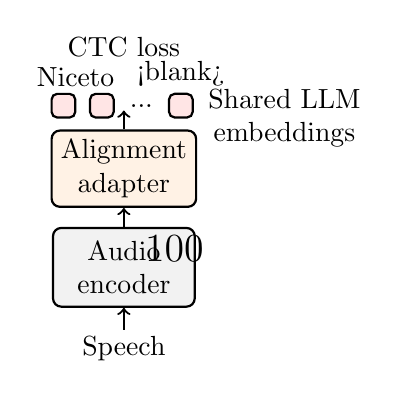
\begin{tikzpicture} [scale=0.8]
        \node(ae) at (0,0) [rectangle, draw=black, fill=gray!10, rounded corners=3pt, thick, minimum width=1.8cm,minimum height=1cm,align=center] {Audio\\encoder};
        \node(freeze) at ([xshift=0.8cm,yshift=0.3cm]ae.center) [rectangle, align=center] {\Large{\ding{100}}};
        \node(fb) at ([yshift=-0.3cm]ae.south) [rectangle, align=center,anchor=north] {Speech};
        \node(aa) at ([yshift=0.3cm]ae.north) [rectangle, draw=black, fill=orange!10, rounded corners=3pt, thick, minimum width=1.8cm,minimum height=0.5cm,align=center,anchor=south] {Alignment\\adapter};
        
        \node(f1) at ([yshift=1.0cm]aa.west) [rectangle, draw=black, fill=red!10, rounded corners=2pt, thick, minimum width=0.3cm, minimum height=0.3cm,align=center,anchor=west] {};
        \node(f2) at ([xshift=0.2cm]f1.east) [rectangle, draw=black, fill=red!10, rounded corners=2pt, thick, minimum width=0.3cm, minimum height=0.3cm,align=center,anchor=west] {};
        \node(f3) at ([xshift=0.075cm]f2.east) [rectangle, draw=white,  thick, align=center,anchor=west] {...};
        \node(f4) at ([xshift=0.075cm]f3.east) [rectangle, draw=black, fill=red!10, rounded corners=2pt, thick, minimum width=0.3cm, minimum height=0.3cm,align=center,anchor=west] {};
        \node(t1) at ([yshift=-0.05cm]f1.north) [rectangle, align=center,anchor=south] {Nice};
        \node(t2) at ([yshift=-0.05cm]f2.north) [rectangle, align=center,anchor=south] {to};
        \node(t4) at ([yshift=-0.05cm]f4.north) [rectangle, align=center,anchor=south] {<blank>};
        \node(se) at ([xshift=0.075cm,yshift=-0.2cm]f4.east) [rectangle, align=center,anchor=west] {Shared LLM\\embeddings};
        \node(ctc) at ([yshift=1.0cm]aa.north) [rectangle, rounded corners=3pt, thick, align=center,anchor=south] {CTC loss};

        
        \draw[->,thick]([yshift=-0.05cm]fb.north)--(ae.south);
        \draw[->,thick](ae.north)--(aa.south);
        \draw[->,thick](aa.north)--([yshift=0.3cm]aa.north);

        
      \end{tikzpicture}
    \end{minipage}
    }
    \subfigure[Shrinking stage]{
    \begin{minipage}[t]{0.45\linewidth}
    \centering
    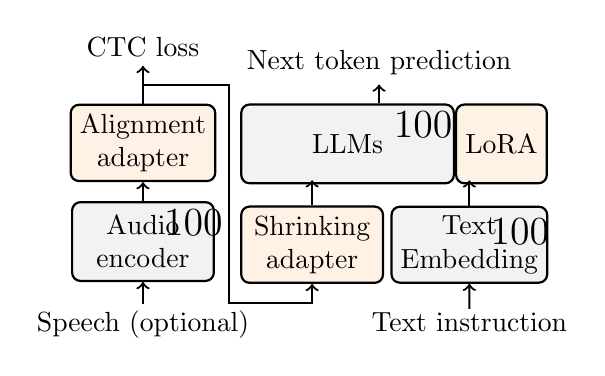
\begin{tikzpicture} [scale=0.8]
        \node(ae) at (0,0) [rectangle, draw=black, fill=gray!10, rounded corners=3pt, thick, minimum width=1.8cm,minimum height=1cm,align=center] {Audio\\encoder};
        \node(freeze) at ([xshift=0.8cm,yshift=0.3cm]ae.center) [rectangle, align=center] {\Large{\ding{100}}};
        \node(fb) at ([yshift=-0.3cm]ae.south) [rectangle, align=center,anchor=north] {Speech (optional)};
        \node(aa) at ([yshift=0.3cm]ae.north) [rectangle, draw=black, fill=orange!10, rounded corners=3pt, thick, minimum width=1.8cm,minimum height=0.5cm,align=center,anchor=south] {Alignment\\adapter};
        \node(ctc) at ([yshift=0.6cm]aa.north) [rectangle,align=center,anchor=south] {CTC loss};
        \node(sa) at ([xshift=0.4cm,yshift=-0.05cm]ae.east) [rectangle, draw=black, fill=orange!10, rounded corners=3pt, thick, minimum width=1.8cm,minimum height=0.5cm,align=center,anchor=west] {Shrinking\\adapter};
        \node(llm) at ([yshift=1.6cm]sa.west) [rectangle, draw=black, fill=gray!10, rounded corners=3pt, thick, minimum width=2.7cm,minimum height=1.0cm,align=center,anchor=west] {LLMs};
        \node(lora) at (llm.east) [rectangle, draw=black, fill=orange!10, rounded corners=3pt, thick, minimum width=1.0cm,minimum height=1.0cm,align=center,anchor=west] {LoRA};
        \node(te) at ([xshift=0.1cm]sa.east) [rectangle, draw=black, fill=gray!10, rounded corners=3pt, thick, minimum width=1.8cm,minimum height=0.5cm,align=center,anchor=west] {Text\\Embedding};
        \node(freeze3) at ([xshift=0.8cm,yshift=0.2cm]te.center) [rectangle, align=center] {\Large{\ding{100}}};
        \node(ti) at ([yshift=-0.3cm]te.south) [rectangle, align=center,anchor=north] {Text instruction};
        \node(freeze2) at ([xshift=1.2cm,yshift=0.3cm]llm.center) [rectangle, align=center] {\Large{\ding{100}}};
        \node(loss) at ([xshift=0.5cm, yshift=0.3cm]llm.north) [rectangle, align=center,anchor=south] {Next token prediction};

        
        \draw[->,thick]([yshift=-0.05cm]fb.north)--(ae.south);
        \draw[->,thick](ae.north)--(aa.south);
        \draw[->,thick](aa.north)--(ctc.south);
        \draw[->,thick](sa.north)--([yshift=0.4cm]sa.north);
        \draw[->,thick](te.north)--([yshift=0.4cm]te.north);
        \draw[->,thick]([yshift=-0.3cm]loss.south)--(loss.south);
        \draw[->,thick]([yshift=-0.1cm]ti.north)--(te.south);

        \draw[->,thick](aa.north)--([yshift=0.3cm]aa.north)--([xshift=0.2cm, yshift=0.3cm]aa.north -| aa.east)--([xshift=0.2cm, yshift=-0.3cm]sa.south -| aa.east)--([yshift=-0.3cm]sa.south)--(sa.south);
      \end{tikzpicture}
    \end{minipage}
    }
    \subfigure[SFT stage]{
    \begin{minipage}[t]{0.20\linewidth}
    \centering
    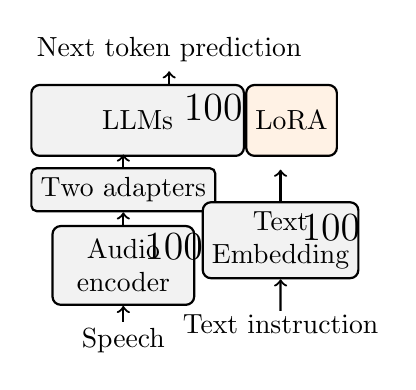
\begin{tikzpicture} [scale=0.8]
        \node(ae) at (0,0) [rectangle, draw=black, fill=gray!10, rounded corners=3pt, thick, minimum width=1.8cm,minimum height=1cm,align=center] {Audio\\encoder};
        \node(freeze) at ([xshift=0.8cm,yshift=0.3cm]ae.center) [rectangle, align=center] {\Large{\ding{100}}};
        \node(fb) at ([yshift=-0.2cm]ae.south) [rectangle, align=center,anchor=north] {Speech};
        \node(aa) at ([yshift=0.2cm]ae.north) [rectangle, draw=black, fill=gray!10, rounded corners=2pt, thick, minimum width=1.8cm,minimum height=0.5cm,align=center,anchor=south] {Two adapters};
        
        \node(llm) at ([yshift=1.1cm]aa.west) [rectangle, draw=black, fill=gray!10, rounded corners=3pt, thick, minimum width=2.7cm,minimum height=0.9cm,align=center,anchor=west] {LLMs};
        \node(lora) at (llm.east) [rectangle, draw=black, fill=orange!10, rounded corners=3pt, thick, minimum width=0.9cm,minimum height=0.9cm,align=center,anchor=west] {LoRA};
        \node(te) at ([xshift=0.1cm,yshift=0.4cm]ae.east) [rectangle, draw=black, fill=gray!10, rounded corners=3pt, thick, minimum width=1.8cm,minimum height=0.5cm,align=center,anchor=west] {Text\\Embedding};
        \node(freeze3) at ([xshift=0.8cm,yshift=0.2cm]te.center) [rectangle, align=center] {\Large{\ding{100}}};
        \node(ti) at ([yshift=-0.4cm]te.south) [rectangle, align=center,anchor=north] {Text instruction};
        \node(freeze2) at ([xshift=1.2cm,yshift=0.2cm]llm.center) [rectangle, align=center] {\Large{\ding{100}}};
        \node(loss) at ([xshift=0.5cm, yshift=0.2cm]llm.north) [rectangle, align=center,anchor=south] {Next token prediction};
       
        \draw[->,thick]([yshift=-0.05cm]fb.north)--(ae.south);
        \draw[->,thick](ae.north)--(aa.south);
        \draw[->,thick](aa.north)--([yshift=0.2cm]aa.north);
        \draw[->,thick](te.north)--([yshift=0.5cm]te.north);
        \draw[->,thick]([yshift=-0.2cm]loss.south)--(loss.south);
        \draw[->,thick]([yshift=-0.1cm]ti.north)--(te.south);
        
      \end{tikzpicture}
    \end{minipage}
    }
      \caption{Training progress of Soundwave. The gray modules are frozen while the orange modules are updated.}
      \label{architecture}
  \end{figure*}

  
\subsection{Online Surveyor}
\label{sec:surveyor}

%The \surveyor~ contains components of \explorer~ and \generator.


\stitle{Exploration}.  The \explorer~ component is designed to give users an intuitive way to interact with the graph database while minimizing the learning curve. %Traditional graph exploration typically relies on query languages, which can require great amount of effort to master. In addition, encountering “supernodes” with exceedingly large numbers of connections can overwhelm users and disrupt the analysis flow.

\begin{figure}
    \centering
    \includegraphics[width=1.0\linewidth]{figures/search.pdf}
    \caption{The Search component of \sys.}
    \label{fig:search_component}
    \vspace*{-2em}
\end{figure}

Traditional graph exploration typically relies on query languages, which can require extra effort to master. We address this by embedding graph queries within interactive UI components. As shown in \reffig{search_component}, the Search module in the \explorer~ helps users pinpoint their initial papers for exploration. Three key interactions are highlighted: ``E1'' searches all nodes containing the ``year'' attribute with a single click; ``E2'' displays a histogram of nodes by ``year'' providing a statistical overview; and ``E3'' filters and retrieves nodes for a specific year (e.g., 2023) by clicking the corresponding histogram bar. These user actions are seamlessly translated into Cypher queries and executed on the underlying graph database.

Furthermore, encountering “supernodes” with exceedingly large numbers of connections can often overwhelm users and disrupt the analysis flow. To address this, we introduce a \statfilter~module that intervenes before displaying all the neighbors. This module can present neighbors either as a histogram, allowing users to quickly overview and multi-select by groups, or as a table, where they can sort by specific attributes and choose the top-k results for further exploration. In \refsec{scenario}, we provide examples showing how this approach streamlines the exploration process.


\stitle{Generation.} Once users finish selecting papers in the \explorer, they can employ the \generator~to convert this explored data into structured reports. By leveraging the natural language understanding and summarization capabilities of LLMs, the \generator~ turns the network of interconnected papers on the canvas into a mind map and, ultimately, a well-formatted narrative report. This process involves three main steps: (1) \textbf{Interpreting User Intentions}: Users describe their desired report in natural language, from which LLM infers which attributes and dimensions of the paper are needed. For instance, if a user asks for a related work section focusing on the paper’s challenges, the LLM may determine that the ``title'' and ``abstract'' attributes and the ``challenges'' dimension are required. Users can review and refine these selections before proceeding. As the dimensions are pre-extracted during the offline \scrapper~ phase, the \generator~ can quickly retrieve them on demand.
(2) \textbf{Generating Mind Maps}: Like a human expert, we prompt the LLM to organize the selected papers into a mind map based on the dimensions mentioned by the users, providing a high-level blueprint for the final report. To accommodate context-size limitations, we adopt an iterative approach that feeds the LLM subsets of the data at a time, gradually constructing the mind map for users to review. % without overwhelming the model.
%The mind map will be shown to the users for checking the correctness and completeness.
(3) \textbf{Writing Reports}: With the mind map in place, the LLM finalizes the literature survey by generating a cohesive report, which can then be downloaded in various formats (e.g., PDF or TeX) to support academic writing.

\begin{figure*}[t!]
    \centering
    \begin{subfigure}[t]{0.24\textwidth}
        \centering
        \includegraphics[width=\textwidth]{fig/overlap_graph_seed0.png}
        \caption{Visualization of 1,000 parties}
        \label{fig:overlap-graph}
    \end{subfigure}
    \hfill
    \begin{subfigure}[t]{0.24\textwidth}
        \centering
        \includegraphics[width=\textwidth]{fig/overlap_distribution.png}
        \caption{Feature overlap ratios}
        \label{fig:feature-overlap}
    \end{subfigure}
    \hfill
    \begin{subfigure}[t]{0.24\textwidth}
        \centering
        \includegraphics[width=\textwidth]{fig/feature_balance_ratio.png}
        \caption{Feature balance ratios}
        \label{fig:feature-skew}
    \end{subfigure}
    \hfill
    \begin{subfigure}[t]{0.24\textwidth}
        \centering
        \includegraphics[width=\textwidth]{fig/matched_ratio_hist.png}
        \caption{Record matched ratios}
        \label{fig:matched-ratio}
    \end{subfigure}    
    \caption{Analysis and visualization of feature distributions and overlaps across real-world databases}
    \label{fig:feature-analysis}
\end{figure*}


This section examines real-world VFL data distributions using the WikiDBs corpus \cite{vogel2024wikidbs}. We begin by introducing the basic settings in Section~\ref{subsec:settings}, define the essential data properties in Section~\ref{subsec:definitions}, and present our results and findings in Section~\ref{subsec:findings}. 

\subsection{Settings}\label{subsec:settings}
\paragraph{Dataset.}
WikiDBs~\cite{vogel2024wikidbs} is currently the largest publicly available corpus of relational databases, extracted from real-world Wikidata. The details of WikiDBs are shown in Table~\ref{tab:wikidbs}. It covers a wide range of domains, such as clinical, finance, sports, etc. Many of these databases (e.g. \texttt{ucl\_clinical\_research\_trials} and \texttt{apnea\_clinical\_research\_db}) are correlated and can be considered potential scenarios for VFL. Each database can be considered a VFL \textit{party}, with pairs of parties sharing correlated features representing potential VFL pairs. 

\begin{table}[h]
    \centering
    \small
    \caption{Statistics of WikiDBs}
    \label{tab:wikidbs}
    \begin{tabular}{cccc}
        \toprule
        \multicolumn{2}{c}{\textbf{Database}} & \multicolumn{2}{c}{\textbf{Table}} \\
        \cmidrule(lr){1-2} \cmidrule(lr){3-4}
        \#Databases & Total \#Tables & Mean \#Rows & Mean \#Cols \\
        \midrule
        100K & 1.6M & 118 & 52.7 \\
        \bottomrule
    \end{tabular}
\end{table}


\paragraph{Configuration.} In our analysis, we focus on two-party VFL, as it not only reflects the characteristics of multi-party VFL but also represents the most common VFL scenario in practice~\cite{liu2024vertical}. Due to the \(O(n^2)\) complexity of evaluating all pairs, we randomly sampled 1,000 databases, generating 1,000,000 pairs from their Cartesian square. Experiments are repeated across 10 random seeds to reduce variance, with mean and variance reported. The results show consistent subset characteristics, demonstrating the robustness of our analysis.

\subsection{Definitions}\label{subsec:definitions}

This subsection delineates the key properties of VFL data distribution. We begin by defining which pairs of databases are considered potential VFL pairs. At the feature level, we assess their overlap and balance by introducing the \textit{feature overlap ratio} and the \textit{feature balance ratio}. In terms of instances, we quantify the proportion of records that can be matched between two parties using shared features, defining this as the \textit{record matched ratio}. The detailed definitions are as follows.

\paragraph{Potential VFL Pairs.} Potential VFL pairs are defined based on database graph connectivity. In this graph, nodes represent databases, and edges connect nodes with tables sharing at least one column. Two databases are considered potential VFL pairs if they belong to the same connected component, indicating they are related through join operations along the connected path.

\paragraph{Record Matched Ratio.} To evaluate how precisely two VFL parties can be aligned based on shared features, we define the \textit{record matched ratio}. For a given table pair, this ratio measures the fraction of records in each table that identically appear in the other. It ranges from $[0, 1]$ and reflects the proportion of records that can be precisely aligned.


\paragraph{Feature Balance Ratio.} To assess the balance in the number of features between two VFL parties, we define the \textit{feature balance ratio} as the small number of columns between the two databases to the large number of columns. The feature balance ratio ranges from $[0, 1]$, where a value of 1 indicates two parties have the same number of features.


\begin{table}[ht]
    \centering
    \small
    \caption{Properties of the database graph across 10 subsets}
    \label{tab:vfl-properties}
    \setlength{\tabcolsep}{3pt}
    \begin{tabular}{ccccc}
        \toprule
        \textbf{Metric} & \textbf{Mean} & \textbf{Std} & \textbf{Min} & \textbf{Max} \\
        \midrule
        \#Connected Components & 3.1 & 0.3 & 3 & 4 \\
        \midrule
       \makecell{Ratio of Non-Neighboring Nodes \\ in Potential VFL Pairs} & 25.4\% & 1.3\% & 23.7\% & 27.7\% \\
        \bottomrule
    \end{tabular}
\end{table}


\begin{table}[ht]
    \centering
    \small
    \caption{The ratio of different VFL data distributions}
    \label{tab:record-matching}
    \setlength{\tabcolsep}{4pt}
    \begin{tabular}{cccc}
        \toprule
        \textbf{VFL Type} & \textbf{Features} & \textbf{Records} & \textbf{Ratio} \\
        \midrule
        Latent VFL & Zero overlap & Zero match & 25.4\% \\
        \midrule
        Fuzzy VFL & Non-zero overlap & Zero match & 70.9\% \\
        Semi-precise VFL & Non-zero overlap & Partial match & 3.5\% \\
        Precise VFL & Non-zero overlap & Full match & 0.2\% \\
        \bottomrule
    \end{tabular}
\end{table}

\subsection{Results and Findings}\label{subsec:findings}


In this subsection, we present our results in Table~\ref{tab:vfl-properties} and Table~\ref{tab:record-matching}, and Figure~\ref{fig:feature-analysis}, followed by four key findings from our analysis of real-world databases.

\begin{tcolorbox}[colback=white, coltitle=black, boxsep=0mm, left=1mm, right=1mm, top=1.5mm, bottom=1mm]
    \textbf{Finding 1}: VFL has a large number of potential real-world applications.
\end{tcolorbox}
To analyze the connectivity between databases, we constructed a graph where each node represents a database, each edge represents shared features between databases, and each color corresponds to a connected component, as visualized in Figure~\ref{fig:overlap-graph}. Table~\ref{tab:vfl-properties} further summarizes the key properties of this graph, showing that the graph of 1,000 parties contains only 3 to 4 connected components. The high connectivity indicated by both the table and figure suggests that VFL has a wide range of potential real-world applications.

\begin{tcolorbox}[colback=white, coltitle=black, boxsep=0mm, left=1mm, right=1mm, top=1.5mm, bottom=1mm]
\textbf{Finding 2}: A substantial portion (25.4\%) of potential VFL pairs have no overlapping features.
\end{tcolorbox}
To analyze feature overlap ratios between potential VFL pairs, we present the distribution of these ratios in Figure~\ref{fig:feature-overlap} and detail the proportion of pairs with zero feature overlap in Table~\ref{tab:vfl-properties}.  Table~\ref{tab:vfl-properties} reveals that among the potential VFL pairs, approximately one-quarter have zero feature overlap. This indicates that many real-world VFL scenarios require methods that can handle latent relationships without relying on shared features. We define a VFL scenario where two parties have no overlapping features but are still correlated as \textit{latent VFL}.

\begin{tcolorbox}[colback=white, coltitle=black, boxsep=0mm, left=1mm, right=1mm, top=1.5mm, bottom=1mm]
\textbf{Finding 3}: Only a small fraction of potential VFL pairs (0.2\%) can be precisely matched.
\end{tcolorbox}
To evaluate the feasibility of record matching in potential VFL pairs, we analyzed the record matched ratios across database pairs. Figure~\ref{fig:matched-ratio} illustrates the distribution of these ratios, and Table~\ref{tab:record-matching} details the ratios for various VFL data distributions. The results reveal that 70.9\% of potential VFL pairs have zero precise record matches, with only 0.2\% achieving full alignment. This indicates that existing VFL algorithms, which assume fully and precisely matched data records (\textit{precise VFL}), may be inadequate for most real-world applications. In practice, there is a need for algorithms capable of handling partial record matching (\textit{semi-precise VFL}) or even scenarios with no record matching (\textit{fuzzy VFL}). This finding aligns with existing VFL studies~\cite{wu2022coupled,nock2021impact,he2024hybrid}, which highlight the rarity of precise matching.

\begin{tcolorbox}[colback=white, coltitle=black, boxsep=0mm, left=1mm, right=1mm, top=1.5mm, bottom=1mm]
\textbf{Finding 4}: Feature distribution across parties exhibits significant imbalance.
\end{tcolorbox}
To evaluate the balance of features between potential VFL pairs, we present the distribution of feature balance ratio in Figure~\ref{fig:feature-skew}. We observe that most database pairs have highly imbalanced feature counts. This imbalance poses challenges for existing VFL algorithms, which typically assume relatively balanced feature distributions across parties for optimal performance. This finding aligns with the observation in~\cite{wu2023vertibench} that real VFL datasets are highly imbalanced w.r.t. feature importance.Imbalanced VFL is defined as a feature balance ratio below 0.5 (66.49\%), while balanced VFL has a ratio above 0.5 (33.51\%).



%%
%% The next two lines define the bibliography style to be used, and
%% the bibliography file.
\bibliographystyle{ACM-Reference-Format}
\bibliography{demo}


\end{document}
\endinput
%%
%% End of file `sample-sigconf.tex'.



\textbf{Insighter Topic Analysis Filtering.} We filter some common generic responses by checking if the response provided by the user is a substring of any of the generic responses, which include responses like ``nothing much" or ``i don't know". In addition, this filter removes all responses that have less than 10 characters, as it is unlikely for an user to describe an quality insight in such brevity. For misspelled responses and other generic responses not caught by this rule-based filtering, a three-shot prompt, which is in Figure \ref{fig:insight_extractor_prompt}, filters out any remaining basic yes or no responses. This prompt also extracts a list of insights from the answer. Using this filtering process, roughly 27.06\% of the answers are kept and used for insight extraction.


\subsection{More Details of User Study}
\label{app.user_study}


\textbf{Informed Consent and Instructions.} Figure~\ref{fig:mturk_consent} shows the informed consent and instructions for the MTurk user study. Participants were informed of the study procedures, potential risks, compensation, future use of information, confidentiality, and voluntary participation. It specifically calls out that participants should not provide any personally identifiable information during this study.

\begin{figure*}[h]
    \centering
    \small
    \resizebox{0.95\textwidth}{!}{
\begin{tcolorbox}[colback=gray!1, colframe=black!50, title=MTurk User Study Informed Consent:]
This AI Chatbot Evaluation task is part of a research study conducted by XXX at XXX University. You will chat with a chatbot for 10-15 minutes and participate in a survey study about your chatbot experience.\\
\\
Purpose\\
The purpose of the research is to evaluate large language model powered chatbots.\\
\\
Procedures \\
First, chat with a chatbot for 10-15 minutes. You are encouraged to engage with the chatbot for up to 15 minutes but can choose to stop engaging with the chatbot at any point of time. Second, immediately after this chatbot interaction, you will complete a survey including questions about the chatbot experience and demographics. This study is voluntary and you can choose to stop or not answer any questions.\\
\\
Participant Requirements \\
Participation in this study is limited to individuals age 18 and older located in the United States. They must have completed at least 1000 HITs and have an approval rate of 99\% or above. Participants must have had prior chatbot experience to participate in this study.\\
\\
Risks\\
The risks and discomfort associated with participation in this study are no greater than those ordinarily encountered in daily life or during other online activities. To minimize the potential risk of a breach of confidentiality, please do not share any personally identifiable information during this study.\\
If you use your personal device for research purpose, there is a risk of incurring data charges. There might be data charges on your device if you are not connected to Wi-Fi.\\
\\
Benefits\\
There may be no personal benefit from your participation in the study. However, we will gain knowledge about the potential pros and cons of different large language models; such knowledge will be valuable to the scientific community and to the public who use these large language models for various tasks.\\
\\
Compensation \& Costs\\
You will be compensated \$5 for your participation in this 30-min study.
There will be no cost to you if you participate in this study.\\
\\
Future Use of Information\\
In the future, once we have removed all identifiable information from your data, we may use the data for our future research studies, or we may distribute the data to other researchers for their research studies.  We would do this without getting additional informed consent from you (or your legally authorized representative). Sharing of data with other researchers will only be done in such a manner that you will not be identified.\\
\\
Confidentiality\\
The data captured for the research does not include any personally identifiable information about you.  Your IP address will not be captured. The study will collect your research data through your use of Amazon MTurk and Qualtrics. These companies are not owned by XXX University. These companies will have access to the research data that you produce and any identifiable information that you share with them while using their product. Please note that XXX University does not control the Terms and Conditions of the companies or how they will use or protect any information that they collect.\\
\\
Payment Confidentiality: Payment methods, especially those facilitated by third-party vendors (such as Visa, Venmo, MTurk, Prolific, Amazon, PayPal), may require that the researchers and/or the vendor collect and use personal information (such as your first and last name, email addresses, phone numbers, banking information) provided by you in order for your payment to be processed. As with any payment transaction, there is the risk of a breach of confidentiality from the third-party vendor. All personal information collected by the researcher will be held as strictly confidential and stored in a password-protected digital file, or in a locked file cabinet, until payments are processed and reconciled. This information will be destroyed at the earliest acceptable time. Personal information held by the third-party vendor will be held according to their terms of use policy.\\
\\
Right to Ask Questions \& Contact Information\\
If you have any questions about this study, you should feel free to ask them by contacting XXX, XXX University, XXX@XXX .  If you have questions later, desire additional information, or wish to withdraw your participation please contact the Principal Investigator by e-mail. If you have questions pertaining to your rights as a research participant; or to report concerns to this study, you should contact the Office of XXX at XXX University.  Email: XXX@XXX . Phone: XXX-XXX -XXXX.\\
\\
Voluntary Participation\\
Your participation in this research is voluntary.  You may discontinue participation at any time during the research activity.  You may print a copy of this consent form for your records.\\

\end{tcolorbox}}
    \caption{Informed consent and instructions provided to MTurk user study participants}
    \label{fig:mturk_consent}
\end{figure*}

\textbf{Demographics.} Table \ref{fig:demographic_mturkers} shows the demographic statistics of the MTurk participants in our user study. Demographic variables reported included gender, race/ethnicity, age, education, and marital status. 
Our participant population is biased towards certain demographic groups, perhaps due to the population distributions of MTurkers during our study period. As a result, all the opinions reflected in this paper are from this specific population, which might be different from current user bases of mainstream LLMs.

\textbf{Payment.} All participants were paid between \$4 and \$6 for their time and participation in this study. This payment rate was determined to be above the US federal minimum wage of \$7.25 per hour. We started with \$4 but then increased to \$6 to facilitate more participation. On average, users spent a total of 25 minutes on our study, corresponding to an average hourly rate of \$12, which is significantly more than the federal minimum wage.

\subsection{Additional Results}
\label{app.add_results}

\textbf{Correlations with User Explicit Rating.} Figure~\ref{fig:scatter_coor} plots the detailed correlations between explicit rating provided by user when asked by \method-Interviewer, and the ratings automatically generated based on user interview responses. Users are significantly more lenient when asked for an explicit rating, giving a lot of perfect 5s. Their responses are more scattered, with a significant fraction of 1 (bad) and 2 (mediocre). It aligns with the findings in UX research that interview is a more effective tool to discover users' true opinions.

\textbf{Interview Examples with Human Annotations.} Figure \ref{fig:chatbot_interview} shows an example of an interview session with human annotations on evaluation dimension, probing occurrences and depth, and previous chat mentioned.

\begin{figure*}[h]
    \centering
    \small
    \resizebox{0.95\textwidth}{!}{
    \begin{tcolorbox}[colback=gray!1, colframe=black!50, title=Example User Experience Interview Session with Human Annotations]
    \textbf{Assistant:} Hello! I'm here to interview you about your experience with the chatbot you just spoke to. Are you ready?\\
    \textbf{User:} yes\\
    
    \textbf{Assistant:} \hl{Great! To start, could you share your overall experience using the ChatBot? How did you feel about the interaction?} \\
    \textit{Dimension: General}\\

    \textbf{User:} My experience with the chatbot was rather informative and engaging.\\
    \textit{Human Dimension Rating: 3 - good}\\

    \textbf{Assistant:} \hl{I'm glad to hear that! Could you tell me more about what made the interaction informative and engaging for you?}\\
    \textit{Dimension: Improvement; Probing Occurrence 1 (Depth 1)}\\

    \textbf{User:} Well it provided me with factual and historical information about the conversations we were having.\\
    \textit{Human Dimension Rating: 3 - good}\\

    \textbf{Assistant:} That's good to know. \hl{Did you feel that the ChatBot understood your questions or requests accurately throughout the conversation?}\\
    \textit{Dimension: Understand}\\

    \textbf{User:} Yes I do,\\
    \textit{Human Dimension Rating for Understand: 3 - good}\\

    \textbf{Assistant:} That's great to hear. \hl{Did the ChatBot successfully meet your needs or solve any problems you had during the conversation?}\\
    \textit{Dimension: Meet Needs}\\

    \textbf{User:} I didn't really have any problems to be solved, {We had a really good conversation about the recent and }\colorbox{teal!30!white}{rare winter storm affecting the south where I live}\\
    \textit{Dimension: Improvement; Previous chat mentioned by user}\\
    \textit{Human Dimension Rating for Meet Needs: 3 - good}\\

    \textbf{Assistant:} Thank you for sharing that. \hl{Did the ChatBot provide coherent, factual, and relevant information} about \colorbox{teal!30!white}{the winter storm and its impact on your area?}\\
    \textit{Dimension: Credibility \& Improvement; Previous chat mentioned by interviewer}\\

    \textbf{User:} Absolutely the chatbot was incredibly relevant and facutal. I was very impressed.\\
    \textit{Human Dimension Rating for Credibility: 3 - good}\\

    \textbf{Assistant:} I'm glad to hear that the information was helpful and accurate. \hl{On a scale of 1 to 5, how satisfied are you with your overall interaction with the ChatBot?}\\
    \textit{Dimension: User Explicit Rating}\\

    \textbf{User:} I would give it a 4.5\\
    \textit{Human Dimension Rating for User Explicit Rating: 4.5}\\

    \textbf{Assistant:} Thank you for your rating. \hl{Is there anything specific that could be improved to make your experience a perfect 5?}\\
    \textit{Dimension: Improvement; Probing Occurrence 2 (Depth 1)}\\

    \textbf{User:} I knew I was chatting with AI, in order for it to be a perfect 5, train AI responses to be a bit less robotic and more humanlike.\\

    \textbf{Assistant:} Thank you for that valuable feedback. \hl{It's important for interactions to feel natural and engaging. Is there anything else you'd like to add or suggest for improving the ChatBot?}\\
    \textit{Dimension: Improvement}\\

    \textbf{User:} None that I can think of at the moment.\\
    
    \textbf{Assistant:} Thank you for your insights and feedback. I appreciate your time and participation in this interview. Have a great day!\\
    
    \textbf{User:} Thank You\\
    
    \textbf{Assistant:} You're welcome! Take care!\\
        
    \end{tcolorbox}}
    \caption{Example interview session with human annotations.}
    \label{fig:chatbot_interview}
\end{figure*}